%%%%%%%%%%%%%%%%%%%%%%%%%%%%%%%%%%%%%%%%%%%%%%%%%%%%%%%%%%%%%%%%%%%%%%%%%%%%%%%%%%%%%%%%%%%%%%%%%%%%%%%
% PACKAGES

\documentclass[a4paper, 11pt]{article}
\usepackage[utf8]{inputenc}
\usepackage[T1]{fontenc}
%\usepackage[catalan]{babel}
\usepackage{amsmath, amssymb, amsthm}
\usepackage[margin=1in]{geometry}
\usepackage{enumerate}
\usepackage{array}
\usepackage{graphicx}
\usepackage{wrapfig}
\usepackage{ragged2e}
\usepackage{subfig}
\usepackage{caption}
\usepackage{subcaption}
\usepackage[dvipsnames]{xcolor}
\usepackage{float}
\usepackage{chngcntr}
\usepackage{ragged2e}
\usepackage{multirow}
\usepackage{vmargin}
\usepackage{hyperref}
\usepackage{url}
\usepackage{fancyhdr}
\usepackage{bigints}
\usepackage{listings}
\usepackage{xcolor,colortbl}
\usepackage[hidelinks]{hyperref}


%%%%%%%%%%%%%%%%%%%%%%%%%%%%%%%%%%%%%%%%%%%%%%%%%%%%%%%%%%%%%%%%%%%%%%%%%%%%%%%%%%%%%%%%%%%%%%%%%%%%%%%
% COLORS

\definecolor{bluebell}{rgb}{0.64, 0.64, 0.82}
\definecolor{atomictangerine}{rgb}{1.0, 0.6, 0.4}
\definecolor{applegreen}{rgb}{0.55, 0.71, 0.0}
\definecolor{frenchblue}{rgb}{0.0, 0.45, 0.73}
\definecolor{darkpastelgreen}{rgb}{0.01, 0.75, 0.24}
\definecolor{darkpastelblue}{rgb}{0.47, 0.62, 0.8}
\definecolor{navy}{rgb}{0,0,128}
\definecolor{codegreen}{rgb}{0,0.6,0}
\definecolor{codegray}{rgb}{0.5,0.5,0.5}
\definecolor{codepurple}{rgb}{0.58,0,0.82}
\definecolor{backcolour}{rgb}{0.95,0.95,0.92}
\definecolor{amaranth}{rgb}{0.9, 0.17, 0.31}
\definecolor{GRAY}{rgb}{0.75, 0.75, 0.75}
\definecolor{deepfuchsia}{rgb}{0.76, 0.33, 0.76}
\definecolor{deepmagenta}{rgb}{0.8, 0.0, 0.8}
\definecolor{funcblue}{rgb}{0.36, 0.57, 0.9}

%%%%%%%%%%%%%%%%%%%%%%%%%%%%%%%%%%%%%%%%%%%%%%%%%%%%%%%%%%%%%%%%%%%%%%%%%%%%%%%%%%%%%%%%%%%%%%%%%%%%%%%
% SETTINGS

% COLOR LINK/REFERENCES
\hypersetup{colorlinks=true,
            linkcolor=blue,
            filecolor=magenta,      
            urlcolor=blue,
            }

% PAGE'S STYLE OF INITIAL PAGES
\fancypagestyle{plain}{
    \lhead[]{} % left part of the header
    \rhead[]{} % right part of the header
    \fancyfoot[]{} % borrow the foot counter page
    \lfoot[]{} % left part of the footpage
    \rfoot[]{} % right part of the footpage
    \renewcommand{\headrulewidth}{0pt} % separator line of the header
    \renewcommand{\footrulewidth}{0.5pt} % separator line of the footpage
}

% PAGE'S STYLE FOR THE THESIS
\fancypagestyle{extended_plain}{
    \lhead[]{Gerard Lahuerta Martín} % left part of the header
    \rhead[]{\leftmark} % right part of the header
    \fancyfoot[]{} % borrow the foot counter page
    \lfoot[]{} % left part of the footpage
    \rfoot[]{\thepage} % right part of the footpage
    \renewcommand{\headrulewidth}{0.5pt} % separator line of the header
    \renewcommand{\footrulewidth}{0.5pt} % separator line of the footpage
}

%%%%%%%%%%%%%%%%%%%%%%%%%%%%%%%%%%%%%%%%%%%%%%%%%%%%%%%%%%%%%%%%%%%%%%%%%%%%%%%%%%%%%%%%%%%%%%%%%%%%%%%
% CODE STYLE


%%%%%%%%%%%%%%%%%%%%%%%%%%%%%%%%%%%%%%%%%%%%%%%%%%%%%%%%%%%%%%%%%%%%%%%%%%%%%%%%%%%%%%%%%%%%%%%%%%%%%%%
% DOCUMENT

\begin{document}
\pagestyle{plain}

% TITLE
\begin{titlepage}
    \centering
    {
\includegraphics[width=0.4\textwidth]{PORTADA/UAB.png}\par}
    \vspace{1cm}
    {\bfseries\LARGE \href{https://www.uab.cat/}{Universitat Autònoma de Barcelona} \par}
    \vspace{2cm}
    {\Large Degree Thesis \par}
    \vspace{2em}
    \hline
    \vspace{1cm}
    {\scshape\Huge \textbf{Improvements of Deterministic Processes through Neural Networks} \par}
    \vspace{1cm}
    \hline
    \vspace{2cm}
    {\Large
    \begin{figure}[h]
    \hspace{-6.5em}
        \begin{minipage}{10cm} \centering % Minipagina para la tabla. 8 cm de ancho
            \begin{tabular}{c}
                Author: \\
                \href{https://github.com/Gerard-Lahuerta}{Gerard Lahuerta Martín}
            \end{tabular}
        \end{minipage}
        \begin{minipage}{10cm} \centering % Minipagina para la tabla. 8 cm de ancho
            \begin{tabular}{c}
                Supervisor: \\
                \href{https://mat.uab.cat/~alseda/}{Dr. Lluís Alsedà Soler}
            \end{tabular}
        \end{minipage}
    \end{figure}\par}
    \vspace{2cm}
    {\scshape 
        \begin{minipage}{10cm} \centering % Minipagina para la tabla. 8 cm de ancho
            A thesis submitted in fulfilment of the requirements
            for the degree of Computational Mathematics and Data Analytics in the
        \end{minipage} 
    \par} 
    \vspace{2em}
    {\scshape\Large \href{https://www.uab.cat/ciencies}{science faculty} \par}
    \vfill
    {\Large June 2024 \par}
\end{titlepage}


\justifying
\newpage
\textcolor{white}{a}
\newpage 

% PRE SECTIONS
\addcontentsline{toc}{section}{Declaration of Authorship}
\section*{Declaration of Authorship}
\newpage
\addcontentsline{toc}{section}{Abstract}
\section*{Abstract}
\newpage
\addcontentsline{toc}{section}{Acknowledgements}
\section*{Acknowledgements}
I would like to express my gratitude to my family for their support throughout my thesis, degree, and my entire life.\\
\textcolor{white}{a}\\
I am especially grateful to my mother, Maria Montserrat, for her encouragement and guidance in facing the challenges of this thesis and my career.\\
\textcolor{white}{a}\\
Thanks to all the peoples that treatme as I was part of their family.\\
\textcolor{white}{a}\\
I also appreciate the encouragement and support of my colleagues.\\
\textcolor{white}{a}\\
Finally, I want to give a special mention to Dr. Lluís Alsedà for guiding me through the thesis and being an inspiration.\\
\textcolor{white}{a}\\
Thank you all for everything. 
\newpage

% CONTENTS
\tableofcontents
\cleardoublepage
\addcontentsline{}{section}{}


\newpage
\addcontentsline{toc}{section}{Preface}
\section*{Preface}


\newpage \pagestyle{extended_plain}
\setcounter{page}{2}
\addcontentsline{toc}{section}{Introducción}
\section*{Introducción}
\newpage

\newpage
\section{Neural Networks} 
A neural Network is made of individual and independent elements connected between them, passing and managing the information through the network formed.\\
In this thesis we will focus on one of the simplest networks, a multilayer perceptron, to test the different methods of optimization.





% MULTILAYER POERCEPTRON
\subsection{Multilayer Perceptron and Perceptron neuron}
One of the simple Neural Networks to analyse is the Multilayer Perceptron\footnote{To obtain more information about Multilayer Perceptron functionability check the following \href{https://en.wikipedia.org/wiki/Multilayer_perceptron}}{link}.\\
It was first proposed by Frank Rosenblat\footnote{Frank Rosenblat, psychologist and father of deep learning, check its \href{https://en.wikipedia.org/wiki/Frank_Rosenblat}{biografy}.} in 1958 (nevertheless its approach did not learn either produce accurate results).
\begin{figure}[h]
    \begin{minipage}{9cm}
       \begin{center}
           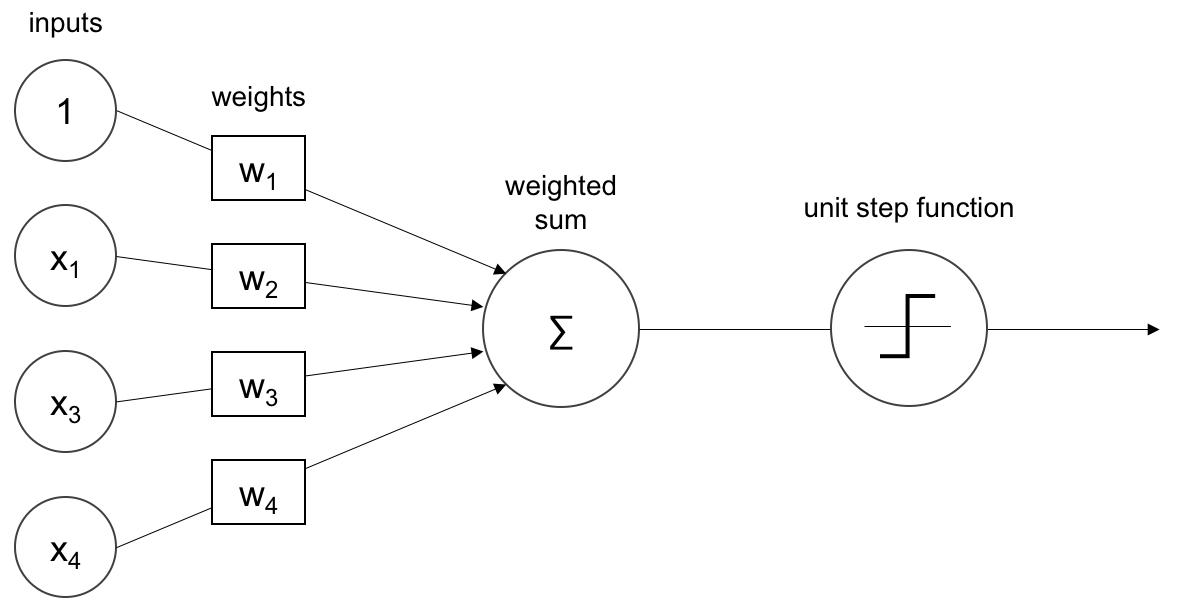
\includegraphics[width = 1 \textwidth]{Neural_Network/perceptron_schema.png}
           \caption{Schema of the Perceptron neuron}
       \end{center} 
    \end{minipage}
    \hspace{1em}
    \begin{minipage}{5cm}
        This Neural Network is formed by elements (the artificial neurons) called \textit{Perceptrons}. This neuron is formed by input, weight and activation functions.\\
        Nevertheless, the most important part of the neuron, and that determines significantly the capabilities of the neuron, is the activation function (which returns the output of the neuron).\\
    \end{minipage}
\end{figure}\\
The traditional activation function used in the Multilayer Perceptron is the Sigmoid: 
$$f(x) = \frac{1}{1+e^{-w\cdot x}},\text{ where: } x,w\in\mathbb{R}^n$$
The Multilayer Perceptron Topology can be splitted into layers of three types:
\begin{figure}[h]
    \begin{minipage}{9cm}
        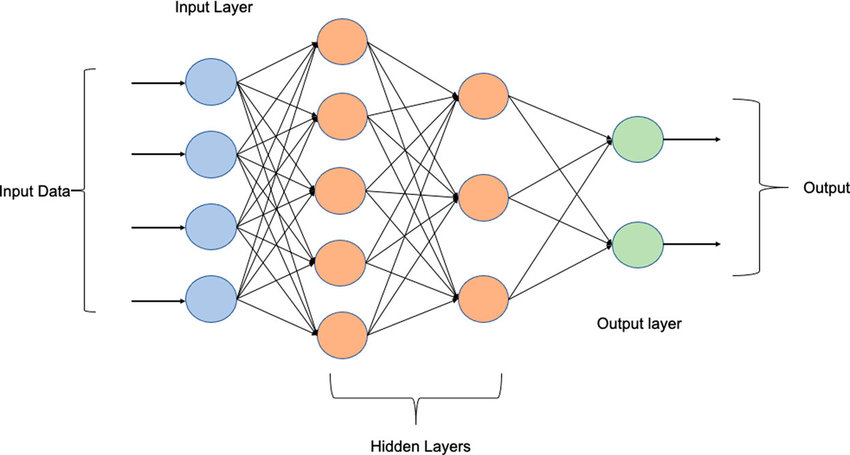
\includegraphics[width = 1 \textwidth]{Neural_Network/Multi-layer-perceptron-MLP-NN-basic-Architecture.png}
        \caption{Schema of the Multilayer perceptron}
    \end{minipage}
    \hspace{1em}
    \begin{minipage}{5cm}
        \begin{itemize}
            \item \textbf{Input Layer}: The initial set of neurons of the Multilayer Perceptron.
            \item \textbf{Output Layer}: The final set of neurons of the Multilayer Perceptron.
            \item \textbf{Hidden Layers}: The set of neurons (in layers) between the input and output layers.
        \end{itemize}
    \end{minipage}
\end{figure}\\
\newpage






% WHY WORKS
\subsection{Why Neural Networks works}
It is important to remark that what gives the capacity of model any system is because we can express everyproblem as a function (no matter if its a classification tasck, probability function, or prediction, regression function).\\
The association between a tasck and a function allow to apply the \textbf{Universal Approximation Theorem}.\\
\hline
\begin{itemize}
    \item \textbf{Definition:} Universal Approximation Theorem.
\end{itemize}  
For any function $f:\mathbb{R}^n \rightarrow \mathbb{R}^m$, with $m,n\in\mathbb{N}$, and a subset $D\subset \mathbb{R}^n$ where $f$ is continuous at all $D$, 
$\exists \{(w_i, b_i, c_i)\}_{i = 0}^k$ that: 
$$f(\vec{x}) - \lim_{k \rightarrow \infty} \sum_{i=0}^{k} c_i \sigma \left( w_i^T \cdot \vec{x} + b_i \right) = 0$$
Where $w_i \in \mathbb{R}^n$, $b_i\in \mathbb{R}$, $c_i \in \mathbb{R}^m$, $\vec{x}\in D$ and $\sigma$ the sigmoid function.\\
\hline\\\vspace{0.5em}
\hspace{-1.6em}The parameters $\{w_i, b_i, c_i\}$ are associated (respectively) with the weights, bias and scale factor of the i-th neuron.\\
Neural Networks essentially use this theorem with a limit number of sigmoid (equal at de number of neurons), consecuently an error of approximation is given.
$$f(\vec{x})-\sum_{i=0}^{k} c_i \sigma \left( w_i^T \cdot \vec{x} + b_i \right) = \epsilon, k \in \mathbb{N}$$
Modeling systems the information of the function shape/tendency is limited or none, making only possible study the problem using data values.\\
This cases hare handle using the \textit{square-norm} metric (or \textit{Mean Squared Error}).\\
\hline
\begin{itemize}
    \item \textbf{Definition:} Square-norm: 
\end{itemize}
Being $f:\mathbb{R}^n \rightarrow \mathbb{R}^m$ function followed by the system.
Being $g:\mathbb{R}^n \rightarrow \mathbb{R}^m$, with $m,n\in\mathbb{N}$, as $g(\vec{x}) = \sum_{i=0}^{k} c_i \sigma \left( w_i^T \cdot \vec{x} + b_i \right)$.\\
Given a dataset $B = \{(\vec{x_i},\vec{y_i})\}_{i=0}^{N}$, with $N \in \mathbb{N}$, where $\forall (\vec{x_i},\vec{y_i}) \in B, \vec{y_i} = f(\vec{x_i})$.
$$\Delta^2 = \frac{1}{N} \sum_{i=0}^{N} \left( \vec{y_i} - g(\vec{x_i}) \right)^2$$
\hline\\\vspace{0.5em}
\hspace{-1.6em}Decreassing the error $\Delta$ implies reducing the error $\epsilon$ because as $\Delta$ decrease the model improves its approximation whereas $\epsilon$ decrease.\\
As the more neurons are added into the Network, the approximation and the training time increases. This increase in training time for the model in cases is not worth it as it represents a minimum improvement of the model.\\
Moreover, the Backpropagation\footnote{The Backpropagation method is an algorithm to modify the internal parameters of a Neural network by using the chain rule, more information in the following \href{https://en.wikipedia.org/wiki/Backpropagation}{link}} method used to train Neural Networks have a complexity that increase the process time exponentially to the number of neurons.\\
Therefore, trying to obtain the ideal topology for solving a problem is a dificult tasck that in many cases resides about trial error.
\newpage 
\section{Neural Networks topology}
The main objective of the study is obtaining a more efficient process using neural networks than the traditional ways that has been used at time.\\
Doing this requires, as has been explained before, a non undertand process to obtain an eficient neural network.\\
Therefore, an observation has done while approaching this problem that could partial solve that non-undertand of what really is doing the neural network and deduce the optimal architecture. 
\subsection{Hypotesis and Proposal}
As has been said before, approaching this problem an intuitive idea apeared. \\
\hline
\begin{itemize}
    \item \textbf{Proposal:} If there is enough information about the system to model, exists an eficient neural network which architecture can be obtained using rules.
\end{itemize}
\hline \\ \vspace{0.5em}
The idea proposed is influenced by the following observations:
\begin{enumerate}
    \item Every deterministic process is a convination of restriccions that can be represented as a function.
    \item Every function can be splitted in domaind which its behavior can be categorized as: periodical, irrational, polinomical.
    \item The periodical, polinomical and irrational functions are continuous in "all"\footnote{In case of irrational functions such as $\sqrt{x}$, it can be interpretated as $f(x) = \left\{ \begin{matrix} 0, x < 0 \\ \sqrt(x), x \geq 0 \end{matrix} \right.$} domain.
    \item All continuous functions can be approximated using the \textbf{Universal Approximation Theorem}.
\end{enumerate}
Moreover, if a function does not follow one of this types of functions, it can be splited by more intervals until each of them can be aproximated by one of this types or even can be approximated using \textit{Fourier Series} or \textit{Taylor series} allowing it to be modeled by periodical and polinomical functions.\\
Therefore, this proposal can be verified reducing it into corroborate the following points:
\begin{enumerate}
    \item Each category of functions mencioned can be modeled using a particular architecture of neural network.
    \item Exists a determined minimum number of data registers were the neural network can be trained.  
\end{enumerate}
To verify the proposal a topological, efficiency and preccision studies is required.

\newpage
\subsection{Study of deterministic process}
\subsection{Conclusions and observations of the results}



\newpage
\begin{thebibliography}{X}
\bibitem{WIKIPEDIA-MLP} \textsc{Wikipedia},
\textit{Multilayer perceptron},\\ \url{https://en.wikipedia.org/wiki/Multilayer_perceptron}
\bibitem{WIKIPEDIA-PERCERPTRON} \textsc{Wikipedia},
\textit{Perceptrón},\\ \url{https://es.wikipedia.org/wiki/Perceptr%C3%B3n}
\bibitem{WIKIPEDIA-ACTIV.FUNCT,} \textsc{Wikipedia},
\textit{Activation function},\\ \url{https://en.wikipedia.org/wiki/Activation_function}
\bibitem{WIKIPEDIA-FRANK} \textsc{Wikipedia},
\textit{Frank Rosenblatt},\\ \url{https://es.wikipedia.org/wiki/Frank_Rosenblatt}
\bibitem{WIKIPEDIA-ACTIVATINGFUNCTION} \textsc{Wikipedia},
\textit{Activating Function},\\ \url{https://en.wikipedia.org/wiki/Activating_function}
\bibitem{WIKIPEDIA-ART.NN} \textsc{Wikipedia},
\textit{Artificial neural network},\\ \url{https://en.wikipedia.org/wiki/Artificial_neural_network}
\bibitem{WIKIPEDIA-NN} \textsc{Wikipedia},
\textit{Neural network},\\ \url{https://en.wikipedia.org/wiki/Neural_network}
\bibitem{WIKIPEDIA-SIGMOID_TEOREM} \textsc{Wikipedia},
\textit{Universal Approximation Theorem},\\ \url{https://en.wikipedia.org/wiki/Universal_approximation_theorem}
\bibitem{WIKIPEDIA-MSE} \textsc{Wikipedia},
\textit{Mean Squared Error},\\ \url{https://en.wikipedia.org/wiki/Mean_squared_error}
\bibitem{WIKIPEDIA-MAE} \textsc{Wikipedia},
\textit{Mean Absolute Error},\\ \url{https://en.wikipedia.org/wiki/Mean_absolute_error}
\bibitem{WIKIPEDIA-CE} \textsc{Wikipedia},
\textit{Cross-Entropy},\\ \url{https://en.wikipedia.org/wiki/Cross-entropy}
\bibitem{WIKIPEDIA-BACKPROP} \textsc{Wikipedia},
\textit{BackPropagation},\\ \url{https://en.wikipedia.org/wiki/Backpropagation}

\bibitem{Dan} \textsc{Dantzig, G.B.} y \textsc{P. Wolfe},
<<Decomposition principle for linear programs>>,
\textit{Operations Research}, \textbf{8}, págs. 101--111, 1960.

\end{thebibliography}
\end{document}
